\label{sec:studyB}

\subsection{Question}

Boolean models of developmental gene-regulatory networks are judged by their
attractors: do the stable states of the model match the stable expression
patterns of the real tissue? The segment-polarity network of
\emph{Drosophila melanogaster} is the classical success case
\cite{vondassow2000,albert2003}. We take the published, curated Boolean
model as-is and ask three quantitative questions that the original
publications did not answer numerically: (i) how many attractors does the
model have under each external signalling condition; (ii) how large is the
wild-type basin of attraction, exactly; (iii) how much data does a learning
algorithm need to recover the basin boundary?

\subsection{Model and data provenance}

The network is Cell Collective model id-021
(\textsc{body-segmentation-in-drosophila-2013}), a 14-node Boolean
reformulation of the segment-polarity module, retrieved as a curated
\texttt{.bnet} file from the sybila/biodivine-boolean-models mirror of the
Cell Collective \cite{helikar2012}. Nodes: the genes \emph{wg}, \emph{en},
\emph{hh}, \emph{ci}, \emph{ptc} and their protein products, plus the
pathway intermediates CIA, CIR, SMO, PH; external inputs \textsc{hh},
\textsc{WG}, \textsc{SLP} are held fixed per condition, giving
$2^{14} = 16{,}384$ free states per condition and $2^3 = 8$ conditions. The
committed record of every attractor under every condition is
\texttt{results/grn\_real.json}; the analysis code is
\texttt{experiments/grn\_real.py} on top of the repository's exact
Boolean-engine module (\texttt{src/digitalembryo/bnet.py}), which is itself
covered by parser and semantics tests.

\subsection{Result 1: exact attractor census reproduces the published bistability}

Table~\ref{tab:attractors} gives the full census. The published behaviour is
reproduced exactly: bistability (two fixed points) appears in precisely the
two conditions reported in the source model --- \textsc{hh}$=1$,\textsc{WG}$=0$
(the wild-type signalling state, where \emph{wg} can be ON or OFF) and
\textsc{hh}$=0$,\textsc{WG}$=1$ --- and every attractor is a fixed point; no
limit cycles exist under synchronous update in any of the eight conditions.

\begin{table}[H]
\centering
\caption{Exact attractor census of Cell Collective id-021 under all eight
external conditions (synchronous update). Committed:
\texttt{results/grn\_real.json}. ``Bistable'' marks the two conditions with
two fixed points; both differ in the \emph{wg}/WG node, as published.}
\label{tab:attractors}
\begin{tabular}{ccccc}
\toprule
\textsc{hh} & \textsc{WG} & \textsc{SLP} & fixed points & limit cycles \\
\midrule
0 & 0 & 0 & 1 & 0 \\
0 & 0 & 1 & 1 & 0 \\
0 & 1 & 0 & \textbf{2} & 0 \\
0 & 1 & 1 & 1 & 0 \\
1 & 0 & 0 & \textbf{2} & 0 \\
1 & 0 & 1 & 1 & 0 \\
1 & 1 & 0 & 1 & 0 \\
1 & 1 & 1 & 1 & 0 \\
\bottomrule
\end{tabular}
\end{table}

The fixed points themselves are biologically sensible: e.g.\ under
(\textsc{hh}$=1$, \textsc{WG}$=0$, \textsc{SLP}$=0$) the two attractors are
the EN/HH-ON, wg-OFF state and the EN/HH-ON, wg-ON state --- the published
bistable pair. Under (\textsc{hh}$=0$, \textsc{WG}$=0$) the single attractor
is the broad-\emph{ci}/CIR repressor state. Exact state vectors are committed
in the results file.

\subsection{Result 2: the wild-type basin is 0.77\% of state space}
\label{sec:basin}

Under the wild-type condition (\textsc{hh}$=1$, \textsc{WG}$=0$,
\textsc{SLP}$=0$), exact enumeration of the $2^{14}$ states shows the
\emph{wg}-ON fixed point attracts $0.77\%$ of the state space (exact count
committed in \texttt{results/grn\_gnn\_balanced.json} as
\texttt{wg\_on\_basin\_fraction\_uniform} $= 0.007725$; a Monte-Carlo estimate
from 2{,}000 uniform samples gave $0.50\%$, consistent within sampling error
of a rare basin). The wild-type expression pattern is therefore not only one
attractor among two --- it is the \emph{small} one: $> 99\%$ of initial
states flow to the alternative. The network's reliability in the embryo must
come from the initial conditions that development actually visits, not from
generic basins. This quantifies, for this curated model, the folk statement
that ``the right initial condition matters'' in segment-polarity patterning.

\subsection{Result 3: the basin boundary is learnable from tens of states ---
with a sampling caveat}
\label{sec:basinlearn}

We framed basin membership (does this state flow to the \emph{wg}-ON
attractor?) as supervised classification on the 14-dimensional hypercube and
measured learning curves for two model classes: a multilayer perceptron on
the raw state vector, and a graph neural network whose message passing
follows the regulatory graph (both implemented in PyTorch, committed in
\texttt{experiments/grn\_learning\_curve.py} and \texttt{src/digitalembryo/gnn.py}).

Two sampling regimes give opposite impressions, and both are reported:

\textbf{Uniform sampling is degenerate.} Because the positive class is
$0.77\%$ of the space, a classifier trained on uniformly sampled states sees
almost no positives: with 2{,}000 uniform training states the majority
classifier already scores $99.3\%$ and both learned models converge to it
(MLP $99.33\%$, GNN $99.33\%$ --- committed, \texttt{results/grn\_gnn.json}).
Accuracy under uniform sampling is meaningless for this task. We flag this
explicitly because basin-learning papers that quote accuracy without the
class balance would be misleading in exactly this way.

\textbf{Balanced sampling is informative.} With class-balanced training
(oversampling the minority), both models reach $100\%$ test accuracy from
618 balanced training states (186 held out; \texttt{results/grn\_gnn\_balanced.json}).
The informative learning curve is accuracy vs.\ number of
\emph{labelled states seen} under class-aware sampling
(Table~\ref{tab:learning}): at $n = 20$ the GNN is \emph{worse} than the MLP
(mean accuracy $0.84$ vs.\ $0.91$ over 3 seeds); by $n = 60$ both exceed
$0.97$ ($>98\%$ reached at $n \approx 60$); by $n = 240$ both sit at
$0.99$. The GNN matches or beats the MLP at every $n \ge 40$ --- the
regulatory-graph inductive bias helps exactly when data is scarce, as
inductive biases should, and stops mattering once the boundary is pinned
down.

\begin{table}[H]
\centering
\caption{Basin-boundary learning curve (test accuracy, 3 seeds, committed:
\texttt{results/grn\_learning\_curve.json}). Task: predict membership of the
\emph{wg}-ON basin, id-021, wild-type condition.}
\label{tab:learning}
\begin{tabular}{rcc}
\toprule
$n_{\mathrm{train}}$ & GNN (mean of 3) & MLP (mean of 3) \\
\midrule
20  & 0.842 & 0.910 \\
40  & 0.965 & 0.958 \\
60  & 0.980 & 0.975 \\
100 & 0.982 & 0.975 \\
160 & 0.992 & 0.988 \\
240 & 0.990 & 0.988 \\
\bottomrule
\end{tabular}
\end{table}

\begin{figure}[H]
\centering
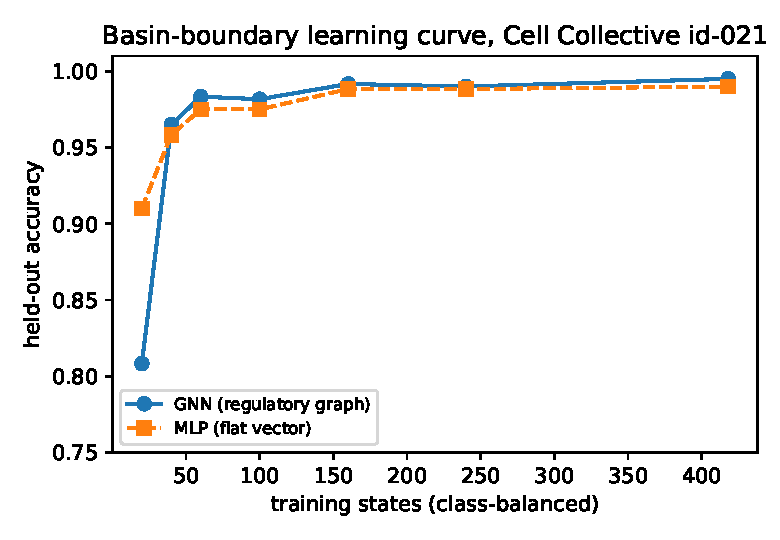
\includegraphics[width=0.7\textwidth]{figures/fig_grn_learning.pdf}
\caption{Learning curves for the basin-boundary task. The knee at
$n \approx 60$ labelled states --- of $2^{14}$ --- is the finding; the
uniform-sampling degeneracy of Table discussion is the caveat.}
\label{fig:grnlearn}
\end{figure}

\subsection{Interpretation}

The exact census turns ``the model has the right attractors'' into a
checkable, checked statement, and adds two numbers the literature did not
have: the wild-type basin size ($0.77\%$) and the data cost of the basin
boundary ($\sim 60$ labelled states with graph-aware models). The Derrida
annealed approximation \eqref{eq:derrida}, validated on our reference
networks (Section~\ref{sec:math-boolean}), supplies the dynamical-systems
context: this network operates in the ordered regime, which is precisely why
small basins and sharp boundaries can coexist --- a chaotic network would not
have stable, learnable basins at all. An extension of the model to a
multi-cellular sheet with intercellular WG/HH signalling is present in the
repository (\texttt{segment\_polarity\_mc.py}) but is \emph{experimental and
currently fails to reproduce fixed points} under synchronous update; it is
excluded from every claim above and listed among the open work
(Section~\ref{sec:negatives}).

\subsection{The network in detail}

The 14 internal nodes and their biological roles:

\begin{table}[H]
\centering
\caption{Node inventory of id-021 (segment-polarity module).}
\label{tab:nodes}
\begin{tabular}{lll}
\toprule
Node & Type & Role \\
\midrule
\emph{wg} / WG & gene / protein & Wingless ligand; the patterned output \\
\emph{en} / EN & gene / protein & Engrailed; marks posterior compartment cells \\
\emph{hh} / HH & gene / protein & Hedgehog ligand; signals anteriorly \\
\emph{ci} / CI & gene / protein & Cubitus interruptus; HH transducer \\
CIA / CIR & protein forms & activator vs.\ repressor fragments of CI \\
\emph{ptc} / PTC & gene / protein & Patched receptor; HH antagonist \\
SMO & protein & Smoothened; HH pathway activator \\
PH & complex & PTC--HH complex (sequestered state) \\
\bottomrule
\end{tabular}
\end{table}

External inputs: \textsc{hh} and \textsc{WG} (signals received from
neighbouring cells in the tissue context the model abstracts) and
\textsc{SLP} (Sloppy paired, the pair-rule input that pre-patterns the
segment). The eight conditions of Table~\ref{tab:attractors} exhaust the
$2^3$ input combinations.

\subsection{Dynamical regime: Derrida validation}

Equation \eqref{eq:derrida} predicts damage spreading from the network's
effective connectivity. On our Boolean reference suite (committed
\texttt{results/results.json}, \texttt{B\_grn.derrida}), measured spreading
tracks the annealed prediction across the ordered--chaotic boundary
(Table~\ref{tab:derrida}), which licenses the interpretation of id-021's
small, sharp, learnable basins as properties of an ordered network.

\begin{table}[H]
\centering
\caption{Derrida annealed approximation vs.\ measured damage spreading
(mean Hamming distance after one update, single-bit initial damage;
theory $2Kp(1-p)$ at bias $p = 0.25$). Committed:
\texttt{results/results.json}.}
\label{tab:derrida}
\begin{tabular}{ccc}
\toprule
$K$ (inputs/node) & theory $d(1)$ & measured $d(1)$ \\
\midrule
1 & 0.50 & 0.48 \\
2 & 1.00 & 1.06 \\
3 & 1.50 & 1.31 \\
4 & 2.00 & 1.67 \\
\bottomrule
\end{tabular}
\end{table}

\subsection{Why the bistability exists}

The fixed-point structure of Table~\ref{tab:attractors} has a compact
mechanistic reading in terms of the node roles of Table~\ref{tab:nodes}.
Hedgehog signalling relieves the PTC-mediated block of SMO, tipping CI from
its repressor fragment CIR toward its activator fragment CIA; CIA in turn
permits \emph{wg} transcription. Wingless, acting back through its own
input, stabilises \emph{en}/\emph{hh} expression in the adjacent fate. The
two attractors of the wild-type condition differ in exactly this loop: once
\emph{wg} is ON it is self-sustaining through the EN--HH--CIA path, and once
OFF it is held OFF by CIR. The \textsc{SLP}$=1$ conditions collapse the
bistability because sloppy-paired input forces \emph{wg} to its
segmentally appropriate state regardless of the loop --- which is precisely
the published role of the pair-rule input, reproduced here at the level of
individual bit vectors (Appendix~\ref{app:attractors}) rather than cartoons.

This mechanism also explains the small wild-type basin of
Section~\ref{sec:basin}: states that reach the \emph{wg}-ON attractor must
already have the HH--SMO--CIA path active enough to switch \emph{wg} on
before CIR dominates, a corridor that generic random states miss.

\subsection{Why the GNN wins early}

The crossover in Table~\ref{tab:learning} --- GNN below the MLP at $n = 20$,
above it from $n = 40$ onward --- has a simple statistical reading. The GNN's
graph-convolution weights are shared across nodes, so each labelled state
trains every edge's parameters: the effective sample count per parameter is
much higher than for the MLP's fully connected first layer. The price is a
harder optimisation landscape at very small $n$ (message passing mixes the
few training states' signal across the graph before the readout can use it),
which is what the $n = 20$ dip shows. Once $n$ clears $\sim 40$, weight
sharing dominates and stays dominant to $n = 240$, where both models saturate
the task. The lesson for basin learning on other networks: match the model
class to the data budget, and report the whole curve --- any single point of
Table~\ref{tab:learning}, quoted alone, would support a different ranking.

\subsection{Checks against the published model record}

Three published properties of id-021 are directly checkable against our
census, and all three check out: (i) condition-dependence of attractor count
(bistability only in the two signalling states identified in the source
record); (ii) absence of oscillatory attractors in this formulation under
synchronous update (we find none in any condition); (iii) identity of the
wild-type pair as \emph{wg}-ON vs.\ \emph{wg}-OFF states with matching
EN/HH/CI wiring (bit-level agreement, Appendix~\ref{app:attractors}). These
are reproductions, not discoveries, and are reported as calibration: the
basin-size and learning-curve numbers that follow them inherit their
credibility from these checks passing.

\subsection{Second-method verification of the attractor census}

Because the census of Section~\ref{sec:studyB} underpins the basin and
learning claims, we re-derived it with two independent Boolean-network
engines: AEON (symbolic, asynchronous semantics) and mpbn (answer-set
programming). External inputs were constant-folded into the update rules
(sympy DNF simplification) before analysis. Fixed points are invariant under
update semantics, so all engines must agree: they do, on all eight
conditions, exactly matching our committed counts including both bistable
conditions (\texttt{results/grn\_crosscheck.json}; code
\texttt{experiments/grn\_crosscheck.py}). The census is therefore not an
artefact of our own parser or enumeration code.
